\documentclass[aspectratio=169]{beamer}
\usepackage[utf8]{inputenc}
\usepackage{tikz}
\usepackage{colortbl}
\usepackage{amsmath}
\usepackage{amssymb}
\usepackage{graphicx}
\usepackage{hyperref}
\usepackage{algorithm}
\usepackage{algpseudocode}
\usepackage{booktabs}
\usepackage{multirow}
\usepackage{xcolor}
\usepackage{listings}
\usepackage{biblatex}

% TikZ libraries
\usetikzlibrary{arrows,automata,positioning,shapes,calc,decorations.pathmorphing,patterns}

% Beamer theme
\usetheme{metropolis}

% Title page info
\title{Probabilistic Algorithms: What, Why, and How}
\subtitle{A Deep Dive into Randomness in Computing}
\author{Sailesh Dahal}
\institute{Kathmandu University}
\date{\today}

% Bibliography
\addbibresource{refs.bib}

% Listings configuration
\lstset{
    language=Python,
    basicstyle=\ttfamily\small,
    breaklines=true,
    frame=single,
    numbers=left,
    numberstyle=\tiny,
    keywordstyle=\color{blue},
    commentstyle=\color{green!60!black},
    stringstyle=\color{red},
    showstringspaces=false
}

\begin{document}

\begin{frame}
  \begin{tikzpicture}[remember picture,overlay]
    \node[anchor=south east, xshift=-5mm, yshift=5mm] at (current page.south east) {
      \includegraphics[width=2cm]{../assets/ku_logo.png}
    };
  \end{tikzpicture}
  \titlepage
\end{frame}

% Outline frame
\begin{frame}{Outline}
  \tableofcontents
\end{frame}

% What are Probabilistic Algorithms?
\section{What are Probabilistic Algorithms?}
\begin{frame}{What is a Probabilistic Algorithm?}
  \begin{block}{Definition}
    An algorithm that makes random choices during execution to influence its behavior or output.
  \end{block}
  \pause
  \begin{itemize}
    \item Output or performance may vary on different runs
    \item Two main types: Las Vegas (always correct, time varies), Monte Carlo (time fixed, may err)
  \end{itemize}
\end{frame}

\begin{frame}{Types of Probabilistic Algorithms}
  \begin{itemize}
    \item \textbf{Las Vegas:} Always correct, random running time
          \pause
    \item \textbf{Monte Carlo:} Fixed running time, may give incorrect result with small probability
          \pause
    \item \textbf{Example:} Randomized Quicksort (Las Vegas)
          \pause
    \item \textbf{Example:} Primality testing (Monte Carlo)
  \end{itemize}
\end{frame}

% Why use Probabilistic Algorithms?
\section{Why Probabilistic Algorithms?}
\begin{frame}{Why Randomness?}
  \begin{block}{Motivation}
    \begin{itemize}
      \item Simpler algorithms
            \pause
      \item Better expected performance
            \pause
      \item Avoid worst-case scenarios
            \pause
      \item Useful for large-scale and distributed systems
    \end{itemize}
  \end{block}
\end{frame}

\begin{frame}{Real-World Motivation}
  \begin{itemize}
    \item Web search (PageRank)
          \pause
    \item Load balancing (power of two choices)
          \pause
    \item Hashing (universal hash functions)
          \pause
    \item Primality testing (Miller-Rabin)
  \end{itemize}
\end{frame}

% How do Probabilistic Algorithms work?
\section{How do Probabilistic Algorithms Work?}
\begin{frame}{How: Randomization in Algorithms}
  \begin{block}{Key Idea}
    Use random choices to influence the algorithm's path or output.
  \end{block}
  \pause
  \begin{itemize}
    \item Random pivot in Quicksort
          \pause
    \item Random walks in graphs
          \pause
    \item Random sampling
  \end{itemize}
\end{frame}

% Example: Randomized Quicksort
\section{Example: Randomized Quicksort}
\begin{frame}{Randomized Quicksort: Step 1 (Initial Array)}
  Consider the array:
  \[
    \renewcommand{\arraystretch}{1.5}
    \begin{array}{|c|c|c|c|c|c|c|c|}
      \hline
      7 & 5 & 9 & 1 & 3 & 4 & 8 & 6 \\
      \hline
    \end{array}
  \]
  \pause
  Suppose the random pivot chosen is \textcolor{red}{5}:
  \[
    \renewcommand{\arraystretch}{1.5}
    \begin{array}{|c|c|c|c|c|c|c|c|}
      \hline
      7 & \cellcolor{red!20}\textcolor{red}{5} & 9 & 1 & 3 & 4 & 8 & 6 \\
      \hline
    \end{array}
  \]
\end{frame}

\begin{frame}{Randomized Quicksort: Step 2 (Partitioning)}
  Partition the array into:
  \begin{itemize}
    \item \textcolor{green!60!black}{Left:} 1, 3, 4 (all $<$ 5)
    \item \textcolor{red}{Middle:} 5 (pivot)
    \item \textcolor{blue}{Right:} 7, 9, 8, 6 (all $>$ 5)
  \end{itemize}
  \pause
  \[
    \renewcommand{\arraystretch}{1.5}
    \begin{array}{|c|c|c|c|c|c|c|c|}
      \hline
      \cellcolor{green!20}\textcolor{green!60!black}{1} & \cellcolor{green!20}\textcolor{green!60!black}{3} & \cellcolor{green!20}\textcolor{green!60!black}{4} & \cellcolor{red!20}\textcolor{red}{5} & \cellcolor{blue!20}\textcolor{blue}{7} & \cellcolor{blue!20}\textcolor{blue}{9} & \cellcolor{blue!20}\textcolor{blue}{8} & \cellcolor{blue!20}\textcolor{blue}{6} \\
      \hline
    \end{array}
  \]
\end{frame}

\begin{frame}{Randomized Quicksort: Step 3 (Left Subarray)}
  Recurse on the left subarray $[1, 3, 4]$.
  \pause
  Suppose the random pivot is \textcolor{red}{3}:
  \[
    \renewcommand{\arraystretch}{1.5}
    \begin{array}{|c|c|c|}
      \hline
      \cellcolor{green!20}\textcolor{green!60!black}{1} & \cellcolor{red!20}\textcolor{red}{3} & \cellcolor{blue!20}\textcolor{blue}{4} \\
      \hline
    \end{array}
  \]
  \pause
  Partition:
  \begin{itemize}
    \item \textcolor{green!60!black}{Left:} 1
    \item \textcolor{red}{Middle:} 3
    \item \textcolor{blue}{Right:} 4
  \end{itemize}
\end{frame}

\begin{frame}{Randomized Quicksort: Step 4 (Right Subarray)}
  Recurse on the right subarray $[7, 9, 8, 6]$.
  \pause
  Suppose the random pivot is \textcolor{red}{8}:
  \[
    \renewcommand{\arraystretch}{1.5}
    \begin{array}{|c|c|c|c|}
      \hline
      \cellcolor{green!20}\textcolor{green!60!black}{7} & \cellcolor{red!20}\textcolor{red}{8} & \cellcolor{blue!20}\textcolor{blue}{9} & \cellcolor{green!20}\textcolor{green!60!black}{6} \\
      \hline
    \end{array}
  \]
  \pause
  Partition:
  \begin{itemize}
    \item \textcolor{green!60!black}{Left:} 7, 6
    \item \textcolor{red}{Middle:} 8
    \item \textcolor{blue}{Right:} 9
  \end{itemize}
\end{frame}

\begin{frame}{Randomized Quicksort: Step 5 (Continue Recursion)}
  Continue recursively on each subarray until all are of length 1.
  \pause
  The final sorted array is:
  \[
    \renewcommand{\arraystretch}{1.5}
    \begin{array}{|c|c|c|c|c|c|c|c|}
      \hline
      1 & 3 & 4 & 5 & 6 & 7 & 8 & 9 \\
      \hline
    \end{array}
  \]
\end{frame}

\begin{frame}[fragile]{Quicksort Implementation (Python)}
  \begin{lstlisting}
import random
def quicksort(arr):
    if len(arr) <= 1:
        return arr
    pivot = random.choice(arr)
    left = [x for x in arr if x < pivot]
    middle = [x for x in arr if x == pivot]
    right = [x for x in arr if x > pivot]
    return quicksort(left) + middle + quicksort(right)
  \end{lstlisting}
\end{frame}

% Analysis: Recurrence and Expectation
\section{Analysis: Recurrence and Expectation}
\begin{frame}{Quicksort Recurrence}
  \begin{block}{Expected Comparisons}
    \[
      T(n) \leq n + \frac{1}{n} \sum_{i=1}^n (T(i-1) + T(n-i))
    \]
    \pause
    Base case: $T(1) = 0$
    \pause
    Solution: $T(n) = O(n \log n)$
  \end{block}
\end{frame}

\begin{frame}{Slick Analysis: Indicator Variables}
  \begin{itemize}
    \item $Q(A)$: Number of comparisons on input $A$
          \pause
    \item $X_{ij}$: Indicator for whether elements $i$ and $j$ are compared
          \pause
    \item $E[Q(A)] = \sum_{i<j} Pr[R_{ij}]$
          \pause
    \item $Pr[R_{ij}] = \frac{2}{j-i+1}$
  \end{itemize}
  \pause
  \begin{block}{Visualization}
    \begin{center}
      % Insert comparison probability diagram here
      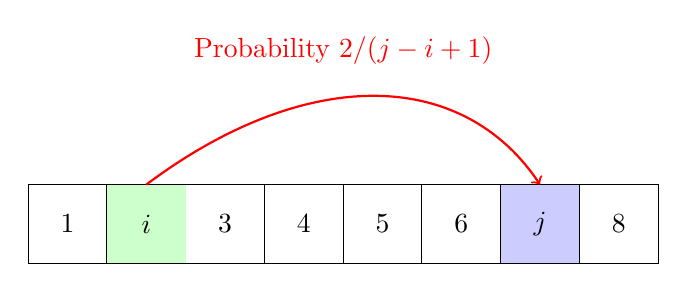
\begin{tikzpicture}[scale=1, every node/.style={scale=1}]
        % Draw array boxes
        \foreach \i in {1,...,8} {
            \draw (\i,0) rectangle (\i+1,1);
            \node at (\i+0.5,0.5) {\i};
          }
        % Highlight i and j
        \fill[green!20] (2,0) rectangle (3,1);
        \fill[blue!20] (7,0) rectangle (8,1);
        \node at (2.5,0.5) {$i$};
        \node at (7.5,0.5) {$j$};
        % Draw arc between i and j
        \draw[thick,red,->] (2.5,1) .. controls (4.5,2.5) and (6.5,2.5) .. (7.5,1);
        \node[red] at (5,2.7) {Probability $2/(j-i+1)$};
      \end{tikzpicture}
    \end{center}
  \end{block}
\end{frame}

\begin{frame}{Harmonic Numbers in Analysis}
  \begin{block}{Harmonic Number}
    $H_n = \sum_{i=1}^n \frac{1}{i} = \Theta(\log n)$
  \end{block}
  \pause
  \begin{block}{Summation in Quicksort}
    $E[Q(A)] \leq 2nH_n = O(n \log n)$
  \end{block}
\end{frame}

% Example: Coin Toss Probability
\section{Example: Coin Toss Probability}
\begin{frame}{Coin Toss Example}
  \begin{block}{Experiment}
    John tosses a biased coin (probability $p$ of heads) to decide whether to wear a tie. If heads, tosses a fair coin to pick red or blue tie.
  \end{block}
  \pause
  \begin{block}{Question}
    What is the probability John wears a red tie on the first day he wears a tie?
  \end{block}
  \pause
  \begin{center}
    % Insert coin toss diagram here
    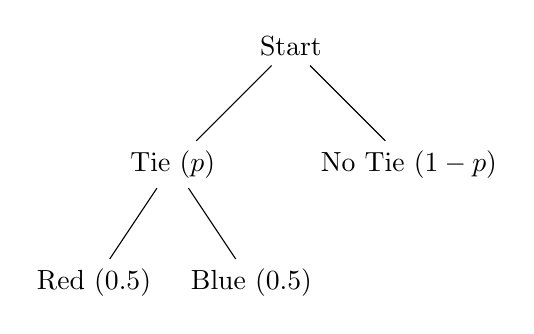
\begin{tikzpicture}[level distance=1.5cm,
        level 1/.style={sibling distance=3cm},
        level 2/.style={sibling distance=2cm}]
      \node {Start}
      child {node {Tie ($p$)}
          child {node {Red (0.5)}}
          child {node {Blue (0.5)}}
        }
      child {node {No Tie ($1-p$)}};
    \end{tikzpicture}
  \end{center}
\end{frame}

% Where do random bits come from?
\section{Random Bits in Practice}
\begin{frame}{Where do Random Bits Come From?}
  \begin{itemize}
    \item Hardware random number generators
          \pause
    \item Pseudo-random number generators (PRNGs)
          \pause
    \item Physical phenomena (thermal noise, radioactive decay)
          \pause
    \item In practice, PRNGs are sufficient for most applications
  \end{itemize}
\end{frame}

% Probabilistic Data Structures
\section{Probabilistic Data Structures}

\begin{frame}{What is a Probabilistic Data Structure?}
  \begin{block}{Definition}
    Data structures that use randomization or probabilistic techniques to achieve space or time efficiency, often allowing for small errors (e.g., false positives).
  \end{block}
  \pause
  \begin{itemize}
    \item Useful for large-scale data, streaming, or approximate answers
    \item Examples: Bloom filter, Count-Min Sketch, HyperLogLog
  \end{itemize}
\end{frame}

\begin{frame}{Bloom Filter: What and Why?}
  \begin{block}{What is a Bloom Filter?}
    A space-efficient, probabilistic data structure for set membership queries.
  \end{block}
  \pause
  \begin{itemize}
    \item Answers: "Is $x$ in the set?"
    \item May return false positives, but never false negatives
    \item Very compact compared to hash sets
  \end{itemize}
\end{frame}

\begin{frame}{How Does a Bloom Filter Work?}
  \begin{enumerate}
    \item Start with a bit array of $m$ bits, all set to 0
          \pause
    \item Use $k$ independent hash functions
          \pause
    \item To add an element, set $k$ bits (one per hash) to 1
          \pause
    \item To check membership, test if all $k$ bits are 1
  \end{enumerate}
\end{frame}

\begin{frame}{Bloom Filter Example}
  Suppose $m=8$ bits, $k=2$ hash functions, and we insert $\{\text{cat}, \text{dog}\}$.
  \pause
  \begin{block}{Bit Array After Insertion}
    \[
      \begin{array}{|c|c|c|c|c|c|c|c|}
        \hline
        1 & 0 & 1 & 1 & 0 & 0 & 0 & 1 \\
        \hline
      \end{array}
    \]
  \end{block}
  \pause
  \begin{itemize}
    \item To check if "cat" is in the set, hash and check the corresponding bits
    \item If all are 1, answer is "possibly in set"; if any is 0, "definitely not in set"
  \end{itemize}
\end{frame}

\begin{frame}{Bloom Filter: Trade-offs}
  \begin{itemize}
    \item \textbf{False positives:} May say "in set" when not
          \pause
    \item \textbf{No false negatives:} Never says "not in set" if it is
          \pause
    \item \textbf{Space efficient:} Much smaller than explicit set
          \pause
    \item \textbf{No deletions:} Standard Bloom filters do not support removing elements
  \end{itemize}
\end{frame}

% References
\begin{frame}[allowframebreaks]{References}
  \printbibliography
\end{frame}

\end{document}
